
\hrule
\section{Abhishek Yadav}
\subsection{Planck's Radiation Law}
\begin{equation}
	\rho(\nu,T)={\frac{8 \pi h \nu^3}{c^3}}  {\frac{1}{\exp_k^{\frac{h \nu}{k_BT}} - 1}}
	\label{eqn:1}
\end{equation}
The Planck's Law describes the energy density of electromagnetic radiation emitted by a black body in thermal equilibrium at a given Temperature T, and there is no net flow of matter or energy between the body and its environment.
The equation~\ref{eqn:1} depicts mathematical form of the Plank's Law. \\
Here \\
$\rho$ - Energy Density \\
$\nu$  - Frequency of radiation emitted \\
$k_B$  -  Boltzmann Constant \\
k      -  Kaniadakis Parameter \\
T      - Temperature \\
h      - Plank Constant \\
The equation shows the fequency dependency of the the energy density ~\cite{meb008}.The figure~\ref{fig:me20b008} shows the graph of variation of energydensity vs frequency.
\begin{figure}[h]
        \begin{center}
		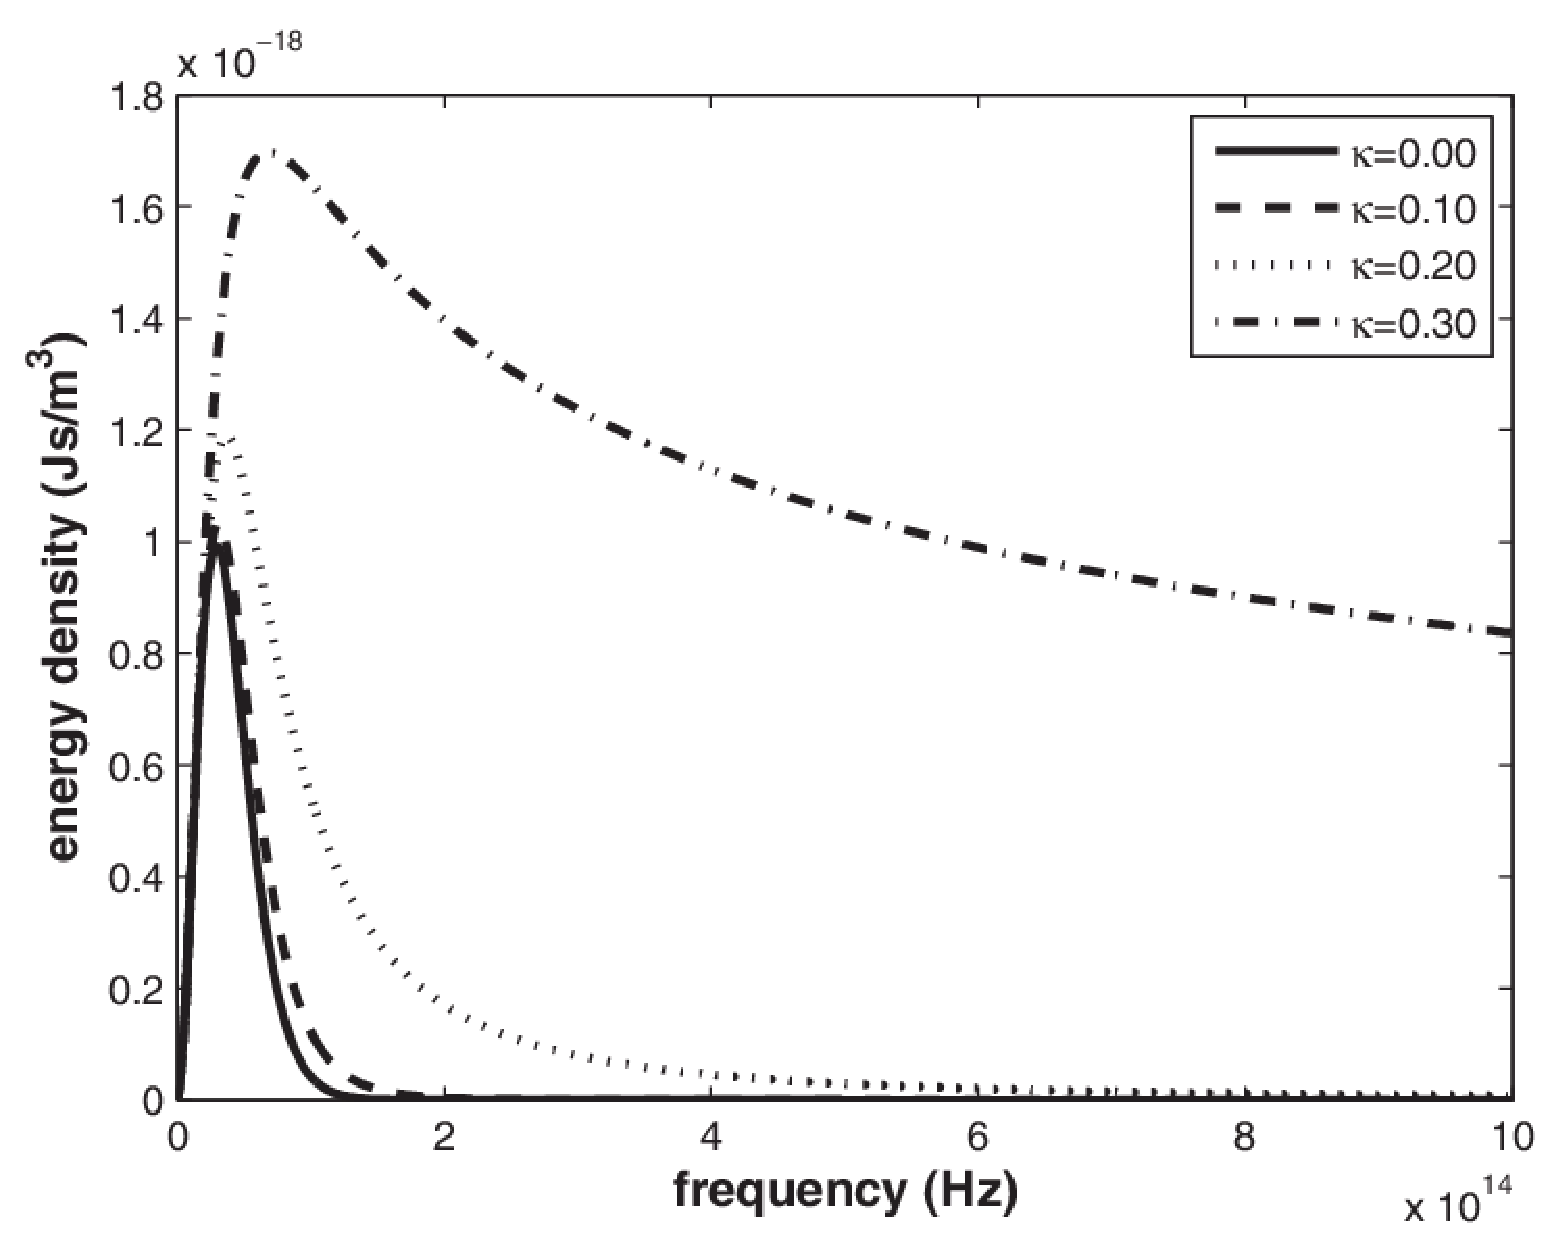
\includegraphics[width=200pt,height=200pt]{me20b008.eps}
		\end{center}
        \caption{Variation of energy density with the frequency, for the different values of Kaniadakis Parameter}
        \label{fig:me20b008}
\end{figure}
\hrule

